第四章给出了无反射数据应满足的代数与谱约束。本章从平面波上的一个 Darboux 因子出发，确定其左右散射归一化，并构造满足全部条件的四点轨道 RHP 解。

\section{Darboux 变换的投影表示}
以下使用文献\cite{LHP2013}式 (3.5)--(3.20) 的 Darboux 定理。将其写为投影形式，可以同时读取无穷远的光场系数和实共振处的介质留数。

\begin{proposition}[已有 Darboux 变换的等价表示]\label{prop:darboux}
设 $(u,v,\eta)$ 为去相位后的经典 HMB 解，$\lambda_1\in\mathbb C^+$ 离开连续谱，$y$ 为 $\lambda_1$ 处非零的同时 Lax 列解。令
\begin{equation}\label{eq:projector}
P=\dfrac{yy^\dagger}{y^\dagger y},\qquad
\delta=\lambda_1-\conj{\lambda_1},\qquad
D(\lambda)=I-\dfrac{\delta}{\lambda-\conj{\lambda_1}}P.
\end{equation}
则新场为
\begin{equation}\label{eq:darbouxfields}
u^{[1]}=u-2\ii\delta P_{12},\qquad
R^{[1]}=D(a)RD(a)^{-1}.
\end{equation}
其中 $R^{[1]}$ 的对角元和负的非对角元分别给出 $\eta^{[1]}$ 与 $v^{[1]}$。变换保持 Hermitian 约化及 Bloch 长度；其逆与行列式为
\begin{equation}\label{eq:Dinverse}
D^{-1}=I+\dfrac{\delta}{\lambda-\lambda_1}P,\qquad
\det D=\dfrac{\lambda-\lambda_1}{\lambda-\conj{\lambda_1}}.
\end{equation}
\begin{equation}\label{eq:Dunitary}
D(a)^{-1}=D(a)^\dagger,\qquad
\left|\dfrac{a-\lambda_1}{a-\conj{\lambda_1}}\right|=1.
\end{equation}
\end{proposition}
\begin{proof}
文献中的一次变换为 $T=\lambda I-S$。取
$S=\conj{\lambda_1}I+(\lambda_1-\conj{\lambda_1})P$，则
$T=(\lambda-\conj{\lambda_1})D$。去掉与 $x,z$ 无关的标量不改变 Lax 交织关系，因此可直接应用该 Darboux 定理。

为确定本节的符号，将 $D=I-\delta P/\lambda+O(\lambda^{-2})$ 代入空间交织关系，比较常数项得
\[
A(u^{[1]})=A(u)-\ii\delta[\sg,P],\qquad
u^{[1]}=u-2\ii\delta P_{12}.
\]
传播交织矩阵 $(D_z+D\widehat V)D^{-1}$ 在 $\lambda=a$ 的留数为 $\ii D(a)RD(a)^{-1}$，给出介质公式。在 $\operatorname{im}P$ 与 $\ker P$ 上，$D$ 分别作用为 $(\lambda-\lambda_1)/(\lambda-\conj{\lambda_1})$ 与 1，故得到逆矩阵、行列式及实 $a$ 上的酉性。于是
\[
(R^{[1]})^\dagger=R^{[1]},\qquad
(R^{[1]})^2=D(a)R^2D(a)^{-1},
\]
约化与 Bloch 长度保持。

投影的微分恒等式也可直接由 Lax 方程核对。若 $B$ 表示对应于变量 $\tau=x$ 或 $z$ 的 Lax 矩阵，则
\begin{equation}\label{eq:Pderivative}
P_\tau=(I-P)B(\lambda_1)P-PB(\conj{\lambda_1})(I-P).
\end{equation}
事实上，对 $yy^\dagger/(y^\dagger y)$ 求导，并用
$y_\tau^\dagger=-y^\dagger B(\conj{\lambda_1})$ 及
$PXP=\tr(XP)P$，得到
\[
P_\tau=B(\lambda_1)P-PB(\conj{\lambda_1})
-P\bigl(B(\lambda_1)-B(\conj{\lambda_1})\bigr)P,
\]
即为 \eqref{eq:Pderivative}。它给出交织矩阵在 $\lambda_1,\conj{\lambda_1}$ 的表观极点相消；完整传播交织关系使用上述文献定理。
\end{proof}

\section{纯虚离散参数的三场解}
取
\begin{equation}\label{eq:imaginarypoint}
\lambda_1=\ii b,\quad b>Q,\quad
\kappa=\sqrt{b^2-Q^2},\quad
W=b+\kappa,\quad h_0=\dfrac{Q}{W}\in(0,1).
\end{equation}
对应谱根为 $\rho_1=\ii\kappa$，单值化点为 $w_1=\ii W$。以常向量 $(1,1)^{\mathsf T}$ 选取背景列
\begin{equation}\label{eq:explicit-y}
s=\kappa[x-F(\ii b)z],\qquad
y=\begin{pmatrix}e^s-h_0e^{-s}\\-h_0e^s+e^{-s}\end{pmatrix}.
\end{equation}
并按 \eqref{eq:projector} 定义 $P,D$。记 $y=(Y_1,Y_2)^{\mathsf T}$、$\Delta=y^\dagger y$，以及恒定相位矩阵 $H=\diag(\ii,-\ii)$。

\begin{proposition}[光滑三场解与同相端态]\label{prop:oneboundary}
由上述 $P$ 定义 $R^{[1]}=D(a)R_\infty D(a)^\dagger$，则
\begin{equation}\label{eq:finalfields}
q=-e^{-\ii\Omega z}\left(Q+4bP_{12}\right),\qquad
p=e^{-\ii\Omega z}(R^{[1]})_{12},\qquad
\eta=(R^{[1]})_{11}.
\end{equation}
是满足边界 \eqref{eq:targetboundary} 的光滑 HMB 解。其去相位介质矩阵为 $HR^{[1]}H^{-1}$，且 Bloch 长度由 \eqref{eq:C} 给出。若 $s=\xi+\ii\nu$，则
\begin{equation}\label{eq:hyperbolic-projector}
P_{12}=
\dfrac{-2h_0\cosh(2\xi)+(1+h_0^2)\cos(2\nu)
+\ii(1-h_0^2)\sin(2\nu)}
{2(1+h_0^2)\cosh(2\xi)-4h_0\cos(2\nu)}.
\end{equation}
分母满足 $\Delta\ge2(1-h_0)^2>0$；固定 $z$ 时，三场趋于端态的速度为 $O(e^{-2\kappa|x|})$。
\end{proposition}
\begin{proof}
列 $y=\Psi_0(w_1)(1,1)^{\mathsf T}$ 同时满足背景 Lax 对。展开其模平方和交叉项得
\begin{align*}
\Delta&=2(1+h_0^2)\cosh(2\xi)-4h_0\cos(2\nu),\\
Y_1\conj{Y_2}
&=-2h_0\cosh(2\xi)+(1+h_0^2)\cos(2\nu)
+\ii(1-h_0^2)\sin(2\nu).
\end{align*}
因此 $\Delta\ge2(1-h_0)^2>0$，并得到 \eqref{eq:hyperbolic-projector}。命题 \ref{prop:darboux} 给出的中间解为
\begin{equation}\label{eq:onefield}
u^{[1]}=Q+4b\dfrac{Y_1\conj{Y_2}}{\Delta},\qquad
R^{[1]}=D(a)R_\infty D(a)^\dagger.
\end{equation}

固定 $z$，$\operatorname{Re}s=\kappa[x-\operatorname{Re}F(\ii b)z]$。故
\begin{equation}\label{eq:Pends}
P_+=\dfrac{1}{1+h_0^2}
\begin{pmatrix}1&-h_0\\-h_0&h_0^2\end{pmatrix},\qquad
P_-=\dfrac{1}{1+h_0^2}
\begin{pmatrix}h_0^2&-h_0\\-h_0&1\end{pmatrix}.
\end{equation}
因为 $2bh_0=Q(1+h_0^2)$，
\[
Q+4b(P_\pm)_{12}=Q-\dfrac{4bh_0}{1+h_0^2}=-Q.
\]
记 $\mathcal D_\pm=I-2\ii bP_\pm/(\lambda+\ii b)$。空间交织关系在端态给出
$\mathcal D_\pm U_Q(\lambda)=U_{-Q}(\lambda)\mathcal D_\pm$。在 $\lambda=a$ 使用
$R_\infty=\ii\eta_0U_Q(a)/a$，得到
$R_\infty^{[1]}=\ii\eta_0U_{-Q}(a)/a$，其对角元为 $\eta_0$，非对角元对应 $v^{[1]}=\ii\eta_0Q/a$。收敛速度由被舍去指数的比值给出，至少为 $O(e^{-2\kappa|x|})$（固定 $z$）。

$\Delta>0$，$a+\ii b\ne0$，所以场表达式在有限实 $x,z$ 上无极点。系统对 $(q,p)\mapsto e^{\ii\phi}(q,p)$ 不变，取 $\phi=\pi$ 即可恢复背景。

恒定共轭 $H$ 恰将光场和极化同时变号，故得到 \eqref{eq:finalfields}。Bloch 约束由实共振处的酉共轭保持。
\end{proof}

若记 $D(a)=(d_{jk})$，则介质分量可写为
\begin{align}
\eta&=\eta_0(|d_{11}|^2-|d_{12}|^2)
+\dfrac{\ii\eta_0Q}{a}(d_{11}\conj{d_{12}}-d_{12}\conj{d_{11}}),\label{eq:etacomponent}\\
e^{\ii\Omega z}p
&=\eta_0(d_{11}\conj{d_{21}}-d_{12}\conj{d_{22}})
+\dfrac{\ii\eta_0Q}{a}(d_{11}\conj{d_{22}}-d_{12}\conj{d_{21}}).\label{eq:pcomponent}
\end{align}
该解属于文献\cite{LHP2013,ZZ2026}的平面波 Darboux 解族。以下确定其在同相端态下的标准 RHP 表示。

\section{四点轨道的标准 RHP}
Darboux 因子在左右端点的极限不同。其作用后的基本解须分别归一化，才能读取透射系数和留数常数。

\begin{lemma}[左右端点的对角归一化]\label{lem:endnormalization}
令 $P_\pm$ 为 \eqref{eq:Pends} 的端点投影，
$\mathcal D_\pm(\lambda)=I-2\ii bP_\pm/(\lambda+\ii b)$，并以 $E_Q=E$、$E_{-Q}=I+\ii Q\sigma_1/w$ 表示两个背景的特征向量矩阵。则
\begin{equation}\label{eq:enddiagonal}
\mathcal D_\pm(\lambda(w))E_Q(w)=E_{-Q}(w)T_\pm(w),
\end{equation}
\begin{align}
T_+&=\diag\left(\dfrac{\rho-\ii\kappa}{\lambda+\ii b},
\dfrac{\rho+\ii\kappa}{\lambda+\ii b}\right),\label{eq:Tplus}\\
T_-&=\diag\left(\dfrac{\rho+\ii\kappa}{\lambda+\ii b},
\dfrac{\rho-\ii\kappa}{\lambda+\ii b}\right).\label{eq:Tminus}
\end{align}
中间解和最终解的 Jost 矩阵分别为
\begin{equation}\label{eq:dressedjost}
\Psi_\pm^{[1]}=D(\lambda)\Psi_0T_\pm^{-1}.
\end{equation}
及 $H\Psi_\pm^{[1]}H^{-1}$，二者具有相同的对角散射矩阵
\begin{equation}\label{eq:onescattering}
S^{[1]}=T_+T_-^{-1}
=\diag\left(\dfrac{\rho-\ii\kappa}{\rho+\ii\kappa},
\dfrac{\rho+\ii\kappa}{\rho-\ii\kappa}\right).
\end{equation}
其 $D_+$ 内的透射零点为
\begin{equation}\label{eq:onezeros}
\zeta_1=\ii(b+\kappa),\qquad
\zeta_2=-\ii(b-\kappa)=h(\conj{\zeta_1}).
\end{equation}
\end{lemma}
\begin{proof}
端态交织关系 $\mathcal D_\pm U_Q=U_{-Q}\mathcal D_\pm$ 表明 $E_{-Q}^{-1}\mathcal D_\pm E_Q$ 为对角矩阵。利用 $2bh_0=Q(1+h_0^2)$、$Q/h_0=b+\kappa$、$Qh_0=b-\kappa$，两个对角因子分别为
\begin{align*}
(\mathcal D_+E_Q)_{11}
&=1-\dfrac{2\ii b}{\lambda+\ii b}\dfrac{1+\ii Qh_0/w}{1+h_0^2}
=\dfrac{\lambda+\ii b-\ii Q/h_0+Q^2/w}{\lambda+\ii b}
=\dfrac{\rho-\ii\kappa}{\lambda+\ii b},\\
(\mathcal D_+E_Q)_{22}
&=1-\dfrac{2\ii b}{\lambda+\ii b}\dfrac{h_0^2+\ii Qh_0/w}{1+h_0^2}
=\dfrac{\rho+\ii\kappa}{\lambda+\ii b}.
\end{align*}
由 $P_-=\sigma_1P_+\sigma_1$ 及 $E_{\pm Q}\sigma_1=\sigma_1E_{\pm Q}$，得到 $T_-=\sigma_1T_+\sigma_1$。

$T_\pm$ 与 $x,z$ 无关且对角，故 \eqref{eq:dressedjost} 满足 Lax 对，其端态为 $E_{-Q}e^{-\ii\theta\sg}$。比较左右两式得到 $S^{[1]}=T_+T_-^{-1}$。共轭 $H$ 将背景恢复为 $Q$，而不改变对角散射矩阵。解 $\rho(w)=\ii\kappa$ 得到 \eqref{eq:onezeros}；$\rho'(\zeta_j)\ne0$ 保证两零点简单。另两点由共轭得到。
\end{proof}

\begin{theorem}[一轨道无反射 RHP]\label{thm:oneRHP}\label{prop:unique-reflectionless}
设 $Q>0,b>Q$，背景参数满足前述条件。用 \eqref{eq:explicit-y} 定义 $P$，则
\begin{equation}\label{eq:explicitM}
M(w)=H\left[(\lambda(w)+\ii b)I-2\ii bP\right]
E_Q(w)
\diag\left(\dfrac{1}{\rho(w)-\ii\kappa},
\dfrac{1}{\rho(w)+\ii\kappa}\right)H^{-1}
\end{equation}
满足定理 \ref{thm:RHP} 的无反射条件。它的两处归一化为 \eqref{eq:Minfty}、\eqref{eq:Mzero}，行列式为 $\gamma$，仅有式 \eqref{eq:onezeros} 及其共轭所指定的列极点；在分支点、轮廓交点和共振原像均有限。其留数常数为
\begin{equation}\label{eq:onec}
c_1=\dfrac{2\ii\kappa}{\rho'(\zeta_1)},\qquad
c_2=-\dfrac{Q^2}{\conj{\zeta_1}^{\,2}}\conj{c_1},
\qquad \rho'(w)=\dfrac{1}{2}\left(1-\dfrac{Q^2}{w^2}\right).
\end{equation}
重构的三个场为 \eqref{eq:finalfields}。
在具有这些留数、两处归一化、换叶约化和行列式，且非极点轮廓处有界的亚纯矩阵类中，该解唯一。
\end{theorem}
\begin{proof}
按式 \eqref{eq:Mdef} 拼接已归一化的 \eqref{eq:dressedjost}。由于 $s_{11}=(T_+)_{11}/(T_-)_{11}$，第一列中的透射系数恰抵消 $T_-$，两侧都得到
$D E_QT_+^{-1}$。再作 $H$ 旋转，得到 \eqref{eq:explicitM}。因此跳跃恒为 $I$。

令 $N=(\lambda+\ii b)I-2\ii bP$，其在 $\operatorname{im}P$ 与 $\ker P$ 的特征值分别为 $\lambda-\ii b$ 和 $\lambda+\ii b$，于是
\[
\det N=\lambda^2+b^2=\rho^2+\kappa^2.
\]
它与两个分母的乘积相消，故 $\det M=\det E_Q=\gamma$。表面上来自 $D$ 的 $\lambda=-\ii b$ 极点已经在 \eqref{eq:explicitM} 中消去；真正剩下的是 $\rho=\pm\ii\kappa$ 的四个列极点。

当 $w\to\infty$ 时，展开为
\[
M=I+\dfrac{H(2\ii bI-4\ii bP-\ii Q\sigma_1+
2\ii\kappa\sg)H^{-1}}{w}+O(w^{-2}).
\]
因 $H$ 共轭把非对角元变号，$\ii M^{(1)}_{12}=-Q-4bP_{12}$，恰为最终去相位光场。利用从 Jost 得到的换叶对称，则 $w\to0$ 时得到 \eqref{eq:Mzero}。共轭对称也由 Jost 约化或 $P^\dagger=P$ 的直接代数验证得到。

在 $w=\pm\ii Q$ 有 $\rho=0$，两个分母均非零；$N,E_Q$ 有限，所以 $M$ 有限，虽然其行列式为零。在 $\pm Q$ 及实共振原像，$\rho$ 为实数，$\rho\pm\ii\kappa$ 不为零，所以同样有限；在共振点 $\gamma>0$，从而可逆。

计算外部零点留数。由 $D(\lambda_1)y=0$，
\[
D(\lambda_1)E_1(\zeta_1)
=-e^{2\ii\theta(\zeta_1)}D(\lambda_1)E_2(\zeta_1).
\]
中间解在该点的相关常数是 $-1$；右乘 $H^{-1}$ 使两列的相对符号改变，所以最终相关常数是 $+1$。又
\[
s_{11}'(\zeta_1)
=\dfrac{\rho'(\zeta_1)}{2\ii\kappa}.
\]
这给出 $c_1$。另一 $D_+$ 点由定理 \ref{thm:RHP} 的配对式 \eqref{eq:cpair} 给出 $c_2$，其余两点由共轭约化给出。

由式 \eqref{eq:onescattering}，$s_{11}(\infty)=s_{11}(0)=1$，其四点表达满足 \eqref{eq:theta-condition}。介质可由 \eqref{eq:RfromM} 重构：在实共振点 $T_+$ 为对角矩阵，与 $\sg$ 对易，代入 $M$ 后即得到 $HD(a)R_\infty D(a)^{-1}H^{-1}$，与 \eqref{eq:finalfields} 一致。

最后证明唯一性。
设 $M,\widetilde M$ 为两个解，考察 $L=M\widetilde M^{-1}$。简单极点处的留数条件可写为
\[
\Res_{w=\zeta_j}M=\lim\limits_{w\to\zeta_j}MA_j,\qquad A_j^2=0,
\]
且 $M,\widetilde M$ 使用同一个 $A_j$。令 $t=w-\zeta_j$，则
\[
M=H_j(w)(I+A_j/t),\qquad
\widetilde M=\widetilde H_j(w)(I+A_j/t),
\]
其中 $H_j=M(I-A_j/t)$ 与 $\widetilde H_j$ 在该点解析。因 $\det(I+A_j/t)=1$ 且 $\gamma(\zeta_j)\ne0$，$\widetilde H_j$ 在该点可逆，于是 $L=H_j\widetilde H_j^{-1}$ 的极点可去。$w=0$ 的主项为相同可逆矩阵 $-\ii Q\sigma_1/w$，故商在那里有限且趋于 $I$。

分支点处的可去性需要利用换叶约化。在 $w_*= \pm\ii Q$，换叶固定该点，故
$M(w_*)=M(w_*)C(w_*)$，$\widetilde M$ 亦同。$C(w_*)$ 有一个 $-1$ 特征空间，两个矩阵都消灭此一维子空间。$\det\widetilde M=\gamma$ 在该点为简单零，故 $\widetilde M(w_*)$ 秩为 1；其伴随矩阵的像就是该核。因此
$M(w_*)\operatorname{adj}\widetilde M(w_*)=0$，商中的行列式简单零被分子抵消。$L$ 在全部有限点可去，无穷远趋于 $I$，Liouville 定理给出 $L=I$。
\end{proof}

\section{一个有理参数例的方程核验}
取参数
\begin{equation}\label{eq:exactparams}
Q=1,\quad b=\dfrac{5}{4},\quad\kappa=\dfrac{3}{4},\quad
a=2,\quad\eta_0=\dfrac{3}{5},\quad\alpha=1,\quad\beta=\dfrac{1}{10}.
\end{equation}
此时 $h_0=1/2$，
\[
F(\ii b)=-\dfrac{3321}{3560}-\dfrac{469}{356}\ii.
\]
写 $T=e^{2\operatorname{Re}s}>0$、$C=e^{2\ii\operatorname{Im}s}$。除去不影响投影的公共因子，$y$ 可以写成 $(TC-1/2,\ 1-TC/2)^{\mathsf T}$，其共轭将 $C$ 替为 $C^{-1}$。因此三个场的去相位形式均为 $T,C$ 的有理函数。链式法则是
\[
\partial_x=2\kappa T\partial_T,\qquad
\partial_z=-2\kappa\operatorname{Re}F\,T\partial_T
-2\ii\kappa\operatorname{Im}F\,C\partial_C.
\]
对这一参数例，投影的分母具体为
\[
\mathcal D(T,C)=\dfrac{5}{4}(T^2+1)-T(C+C^{-1}),
\]
且
\[
P=\dfrac{1}{\mathcal D}
\begin{pmatrix}
(TC-\dfrac{1}{2})(T/C-\dfrac{1}{2})&(TC-\dfrac{1}{2})(1-T/(2C))\\
(1-TC/2)(T/C-\dfrac{1}{2})&(1-TC/2)(1-T/(2C))
\end{pmatrix}.
\]
在实际参数曲面 $T>0,|C|=1$ 上，$\mathcal D$ 是两个模平方之和，严格为正。实共振点的 Darboux 因子为
\[
D(a)=I-\dfrac{50+80\ii}{89}P,\qquad
R_\infty=\begin{pmatrix}\dfrac{3}{5}&\dfrac{3\ii}{10}\\
-\dfrac{3\ii}{10}&-\dfrac{3}{5}\end{pmatrix}.
\]
所以 $u=-1-5P_{12}$，$v=(D(a)R_\infty D(a)^\dagger)_{12}$，
$\eta=(D(a)R_\infty D(a)^\dagger)_{11}$，均为 $T,C$ 的明确有理表达式。
有理运算中以 $C^{-1}$ 和 $-\ii$ 分别替换共轭的 $C$ 与 $\ii$，并保持 $T$ 不变。

三条原 PDE 在去相位变量中的残差分别为
\begin{align*}
\mathcal E_q&=u_z-\ii\Omega u-\ii\alpha(u_{xx}/2+u\conj u\,u)
-\beta(u_{xxx}+6u\conj u\,u_x)-2v,\\
\mathcal E_p&=v_x-2\eta u+2\ii av,\qquad
\mathcal E_\eta=\eta_x+\conj u\,v+u\conj v,
\end{align*}
将上述有理表达式代入，精确符号化简给出 $\mathcal E_q=\mathcal E_p=\mathcal E_\eta=0$，以及 $|v|^2+\eta^2=9/20$。由于 $\mathcal D>0$，清分母不改变原等式。这一计算核对了所列参数下的三场公式；一般参数的方程性质已由命题 \ref{prop:oneboundary} 保证。


\section{多次变换与数值例}
取互异的 $\lambda_j\in\mathbb C^+$，并使其避开背景连续谱。定义背景列
$y_j^{(0)}=\Psi_0(\lambda_j)c_j^{(0)}$，其中 $c_j^{(0)}\ne0$。按顺序定义
\begin{align}
y_j^{(j-1)}&=D_{j-1}(\lambda_j)\cdots D_1(\lambda_j)y_j^{(0)},\label{eq:Nrecursion}\\
P_j&=\dfrac{y_j^{(j-1)}(y_j^{(j-1)})^\dagger}
{(y_j^{(j-1)})^\dagger y_j^{(j-1)}},\qquad
D_j(\lambda)=I-\dfrac{\lambda_j-\conj{\lambda_j}}
{\lambda-\conj{\lambda_j}}P_j,\nonumber\\
u^{[j]}&=u^{[j-1]}-2\ii(\lambda_j-\conj{\lambda_j})(P_j)_{12},\nonumber\\
R^{[j]}&=D_j(a)R^{[j-1]}D_j(a)^\dagger.\label{eq:Nmedium}
\end{align}
因各 $D_k(\lambda_j)$ 可逆，输入列不为零，投影分母严格正；实 $a$ 上的酉性保持 Bloch 长度。逐次应用命题 \ref{prop:darboux}，得到新的 HMB 解。

对互异纯虚参数 $\lambda_j=\ii b_j$、$b_j>Q$，各种子常向量均取 $(1,1)^{\mathsf T}$ 时，每一步的两个端态同时变号。事实上，前面各变换在新的 $\lambda_j$ 可逆，故不会消灭种子的主导端态特征向量；由端态交织关系，该向量变为新背景的相应特征向量，下一步投影因而仍为式 \eqref{eq:Pends} 的相应背景符号版本。归纳得到最终共同端态为 $(-1)^NQ$，将光场和极化乘 $(-1)^N$ 即恢复指定端态。下面的二重例子取 $Q=1$、$b_1=1.5$、$b_2=1.9$。

一般复谱参数通常导致不同的左右端态相位。式 \eqref{eq:Nrecursion}--\eqref{eq:Nmedium} 给出基于 Darboux 定理的递推解；将其对应到同相背景的标准 RHP，还须确定左右归一化、全部范数常数以及式 \eqref{eq:theta-condition}。一轨道的完整对应已由定理 \ref{thm:oneRHP} 给出。


作为一重与二重变换的数值核对，取 $Q=1,a=2,\eta_0=0.6,\alpha=1,\beta=0.1$，一重谱点 $1.5\ii$，二重再加入 $1.9\ii$。采用 60 位十进制精度，分别对显式表达式求导，未使用 PDE 右侧生成导数。采样点为
$(-1.2,-0.35)$、$(0,0)$、$(0.37,0.21)$、$(1.4,-0.1)$ 和 $(2.3,0.6)$。

\begin{table}[htbp]
\centering
\caption{三场方程与 Bloch 约束的最大绝对残差（五点采样，60 位精度）}
\begin{tabular}{ccccc}
\toprule 重数 & 光场方程 & 极化方程 & 反转方程 & Bloch 偏差\\\midrule
1 & $1.02\times10^{-60}$ & $3.14\times10^{-61}$ & $7.47\times10^{-62}$ & $3.89\times10^{-62}$\\
2 & $1.75\times10^{-59}$ & $2.66\times10^{-60}$ & $9.34\times10^{-61}$ & $1.95\times10^{-61}$\\
\bottomrule
\end{tabular}
\end{table}
表中数值为最大绝对残差的向上舍入值。固定 $z=0.21$、在 $x=\pm30$ 检查三个端态，一重误差均小于 $5.1\times10^{-29}$，二重误差均小于 $2.8\times10^{-28}$。另对显式 RHP 矩阵检查了两留数、两种谱对称、空间 Lax 方程、行列式与两共振原像的介质重构，全部误差小于 $7.0\times10^{-61}$。这些有限采样用于检验显式表达式与解析推导的一致性；解的方程性质由前述证明及文献中的 Darboux 定理保证。

图 \ref{fig:one}、\ref{fig:two} 展示对应的三场分布；此时 Bloch 长度平方为 $0.45$。图像由投影表达式在双精度网格上求值，表中残差则采用任意精度微分计算。

\begin{figure}[htbp]
\centering
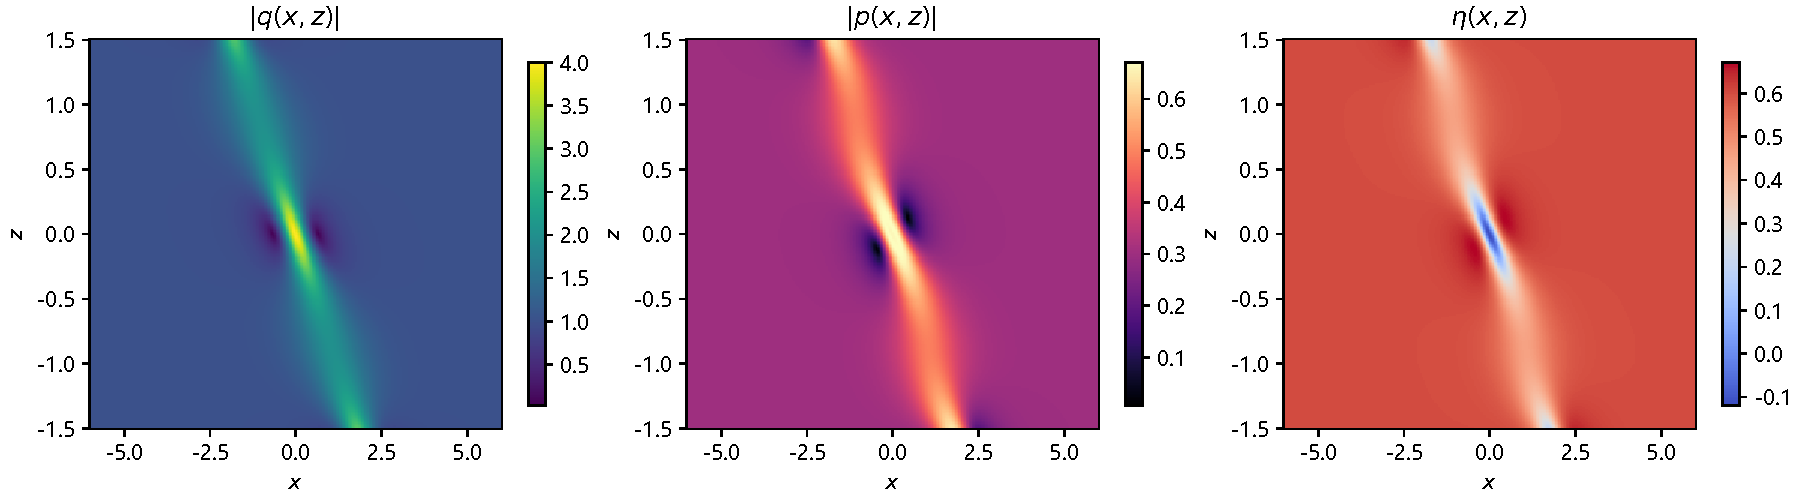
\includegraphics[width=\textwidth]{figures/one-soliton-fields.pdf}
\caption{一组四点谱轨道的三场图像。$Q=1,a=2,\eta_0=0.6,\alpha=1,\beta=0.1,b=1.5$；颜色分别表示 $|q|,|p|,\eta$。纵轴为传播变量 $z$，横轴为推迟时间 $x$。}
\label{fig:one}
\end{figure}
\begin{figure}[htbp]
\centering
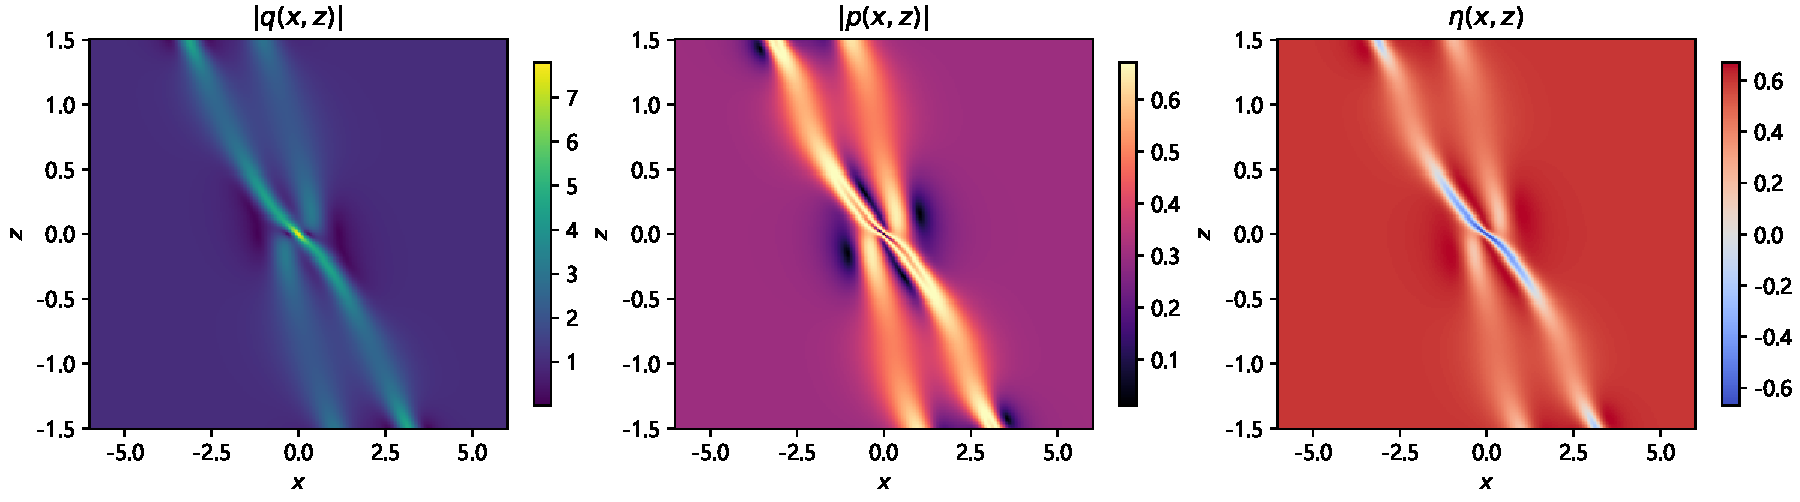
\includegraphics[width=\textwidth]{figures/two-soliton-fields.pdf}
\caption{同一背景下二次 dressing，谱点为 $1.5\ii,1.9\ii$。两个种子常向量均为 $(1,1)^{\mathsf T}$，三场由式 \eqref{eq:Nrecursion}--\eqref{eq:Nmedium} 递推得到。}
\label{fig:two}
\end{figure}
